\documentclass[a4paper,12pt]{article}

\usepackage[T2A]{fontenc}			
\usepackage[utf8]{inputenc}			
\usepackage[english,russian]{babel}	

\usepackage[
bookmarks=true, colorlinks=true, unicode=true,
urlcolor=black,linkcolor=black, anchorcolor=black,
citecolor=black, menucolor=black, filecolor=black,
]{hyperref}

\usepackage{color}
\usepackage{caption}
\DeclareCaptionFont{white}{\color{black}}
\DeclareCaptionFormat{listing}{\colorbox{white}{\parbox{\textwidth}{#1#2#3}}}
\captionsetup[lstlisting]{format=listing,labelfont=white,textfont=white}

\usepackage{amsmath,amsfonts,amssymb,amsthm,mathtools} 
\usepackage{wasysym}

\usepackage{graphicx}
%\usepackage[cache=false]{minted}
\usepackage{cmap}
\usepackage{indentfirst}

\usepackage{listings} 
\usepackage{fancyvrb}

\usepackage{geometry}
\geometry{left=2cm}
\geometry{right=1.5cm}
\geometry{top=1cm}
\geometry{bottom=2cm}

\setlength{\parindent}{5ex}
\setlength{\parskip}{0.5em}

\usepackage{pgfplots}

\usepackage{longtable}

\begin{document}
	\lstset{ %
		language=C,                 % выбор языка для подсветки (здесь это С)
		basicstyle=\small\sffamily, % размер и начертание шрифта для подсветки кода
		numbers=left,               % где поставить нумерацию строк (слева\справа)
		numberstyle=\tiny,           % размер шрифта для номеров строк
		stepnumber=1,                   % размер шага между двумя номерами строк
		numbersep=5pt,                % как далеко отстоят номера строк от подсвечиваемого кода
		backgroundcolor=\color{white}, % цвет фона подсветки - используем \usepackage{color}
		showspaces=false,            % показывать или нет пробелы специальными отступами
		showstringspaces=false,      % показывать или нет пробелы в строках
		showtabs=false,             % показывать или нет табуляцию в строках
		frame=single,              % рисовать рамку вокруг кода
		tabsize=2,                 % размер табуляции по умолчанию равен 2 пробелам
		captionpos=t,              % позиция заголовка вверху [t] или внизу [b] 
		breaklines=true,           % автоматически переносить строки (да\нет)
		breakatwhitespace=false, % переносить строки только если есть пробел
		escapeinside={\%*}{*)}   % если нужно добавить комментарии в коде
	}
	
	% Титульный лист
	\begin{figure}[h!]
		\begin{center}
			{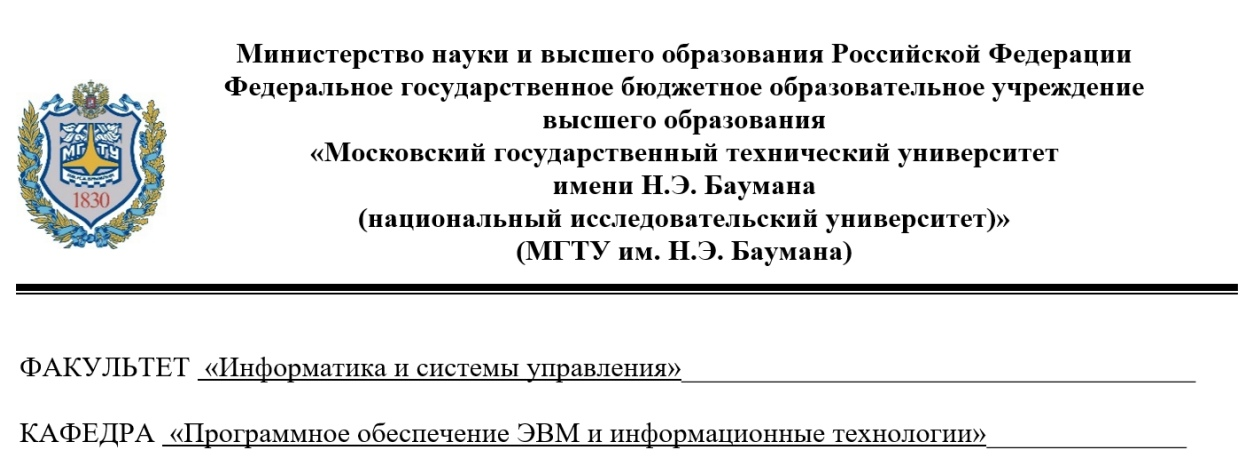
\includegraphics[scale = 0.4]{titul.jpg}}
			\label{titul}
		\end{center}
	\end{figure}
	
	\vspace*{15mm} 
	
	\huge
	\begin{center}
		Дисциплина: <<Моделирование>>
	\end{center}
	
	\begin{center}
		Лабораторная работа №4
	\end{center}

	
	\huge
	\begin{center}
		Тема работы:\\
		<<Моделирование работы обслуживающего аппарата>>
	\end{center}
	\vspace*{25mm} 
	
	\large
	\begin{flushright}
		Студент: Левушкин И. К. \\
		Группа: ИУ7-72Б \\
		Преподаватель: Рудаков И. В. \\
	\end{flushright}
	
	\vspace*{25mm}
	\begin{center}
		Москва, 2020 г.  
	\end{center}
	\thispagestyle{empty}
	
	
	\newpage
	
	\section*{Задание}
	
	Необходимо промоделировать систему, состоящую из генератора, памяти, емкости $L$ и обслуживающего аппарата. Генератор выдает сообщения, распределенные по равномерному закону, они приходят в память (FIFO) и выбираются по закону второй лабораторной работы (Экспоненциальное распределение). Параметры задаются. Необходимо определить оптимальную длину очереди при которой не будет потерянных сообщений, используя 2 принципа: $\Delta t$-метод и событийный метод.
	
	\newpage
	
	\section*{Формализация}
	
	\subsection*{Управляющая программа имитационной модели}
	
	\textit{Управляющая программа} имитирует алгоритм взаимодействия отдельных устройств системы.
	
	Она реализуется двумя принципами:
	
	\begin{itemize}
		\item Принцип $\Delta t$
		\item Событийный принцип
	\end{itemize}

	{\bf Принцип $\Delta t$.}
	
	Принцип $\Delta t$ заключается в последовательном анализе состояний всех блоков в момент $t + \Delta t$ по заданному состоянию блоков в момент $t$. При этом новое состояние блоков определяется в соответствии с их алгоритмическим описанием с учетом действующих случайных факторов, задаваемых распределениями вероятности. В результате такого анализа принимается решение о том, какие общесистемные события должны имитироваться программной моделью на данный момент времени. 
	
	Основной {\bf недостаток} этого принципа: значительные затраты машинного времени на реализацию моделирования системы. А при недостаточно малом $\Delta t$ появляется опасность пропуска отдельных событий в системе, что исключает возможность получения адекватных результатов при моделировании.
	
	{\bf Достоинство}: равномерная протяжка времени.
	
	{\bf Событийный принцип.}
	
	Характерное свойство систем обработки информации то, что состояние отдельных устройств изменяются в дискретные моменты времени, совпадающие с моментами времени поступления сообщений в систему, временем поступления окончания задачи, времени поступления аварийных сигналов и т.д. Поэтому моделирование и продвижение времени в системе удобно проводить, используя событийный принцип, при котором состояние всех блоков имитационной модели анализируется лишь в момент появления какого-либо события. Момент поступления следующего события определяется минимальным значением из списка будущих событий, представляющего собой совокупность моментов ближайшего изменения состояния каждого из блоков системы. 
	
	{\bf Недостаток} событийного принципа: (самостоятельная обработка).
	
	\newpage
	
	Ниже приведена схема событийного принципа.
	
	\begin{figure}[h!]
		\begin{center}
			{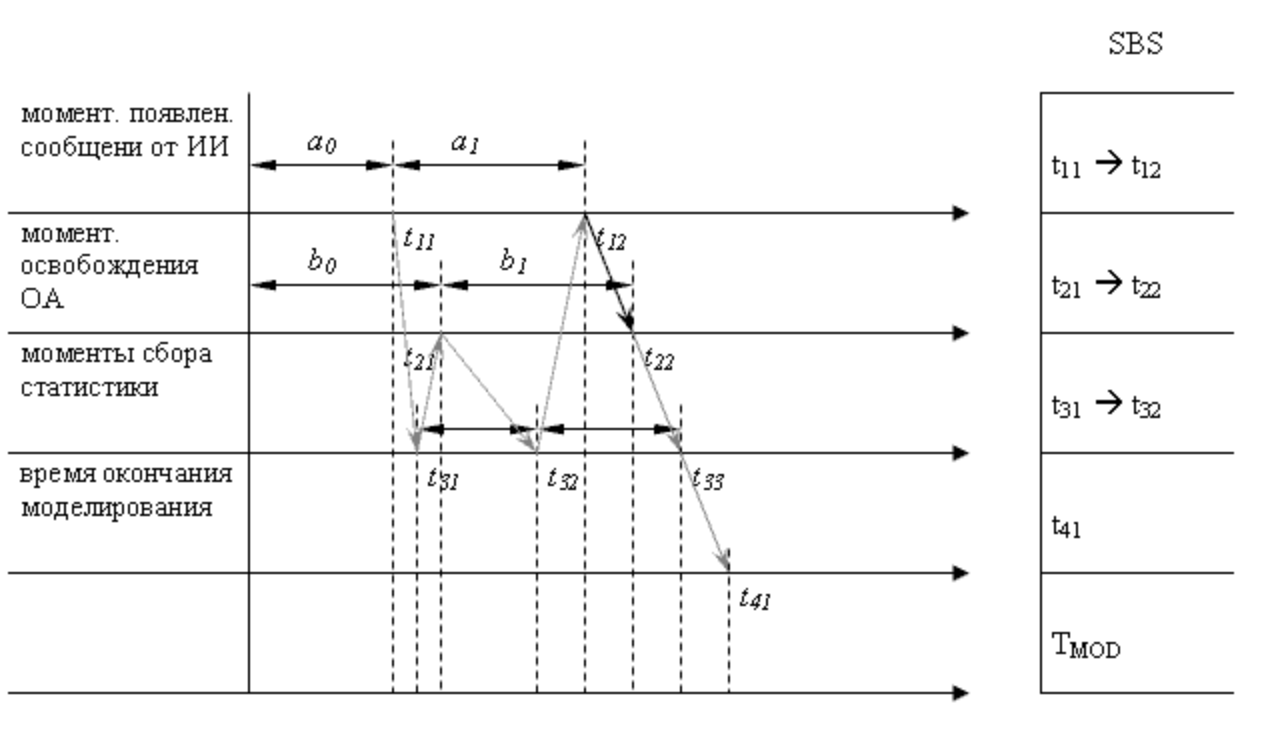
\includegraphics[scale = 0.6]{sob.png}}
			\label{ris:sob}
		\end{center}
		\caption{Схема событийного принципа.}
	\end{figure}

	Где 
	\begin{itemize}
		\item Первая ось: момент появления сообщений;
		\item Вторая ось: момент освобождения обслуживающего аппарата;
		\item Третья ось: момент сбора статистики;
		\item Четвертая ось: время окончания моделирования;
		\item Пятая ось: текущее время;
		\item $t_{11}$, $t_{12}$ – моменты появления сообщений на выходе генератора; \item $b_1$ – интервал времени обслуживания первого сообщения;
		\item $t_{3n}$ – моменты сбора статистики;
		\item $t_{41}$ – момент окончания моделирования;
		\item SBS – список будущих событий.
	\end{itemize}

	Таким образом, анализ состояния блоков происходит только во времена $t_{11}, t_{31}, t_{21}, t_{32}, t_{12}, t_{22}, t_{33}, t_{41}$, соответственно (серая ломаная линия на схеме событийного принципа).
	
	\newpage
	
	Ниже приведена схема управляющей программы имитационной модели.
	
	\begin{figure}[h!]
		\begin{center}
			{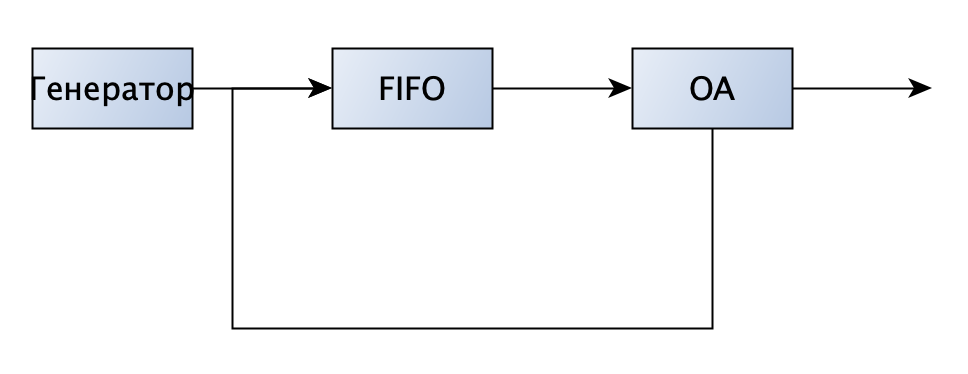
\includegraphics[scale = 0.6]{imit.png}}
			\label{ris:imit}
		\end{center}
		\caption{Схема управляющей программы имитационной модели.}
	\end{figure}

	Откуда видно, что Обслуживающий Аппарат может отправлять заявку на повторную обработку (ставит в очередь). Это происходит с определенной задаваемой вероятностью $Q$.
	
	Как было сказано в условии лабораторной работы, генератор создает заявки по равномерному закону. Это значит, что время, через которое будет создана следующая заявка, распределено равномерно на интервале от $[a, b]$. Аналогичная ситуация с обслуживающим аппаратом, обрабатывающим заявки по экспоненциальному закону (задается параметр $\lambda$).
	
	Буферная память работает по принципу очереди (FIFO - первый вошел, первый вышел).
	
	\section*{Результаты работы программы}
	
	Ниже приведены результаты работы программы при следующих параметрах:
	
	\begin{itemize}
		\item $a$ = 1;
		\item $b$ = 10;
		\item $\lambda$ = 1;
		\item Вероятность повторной обработки заявки = 0;
		\item Количество заявок = 1000;
	\end{itemize}

	\newpage

	\begin{figure}[h!]
		\begin{minipage}[b]{0.32\textwidth}
			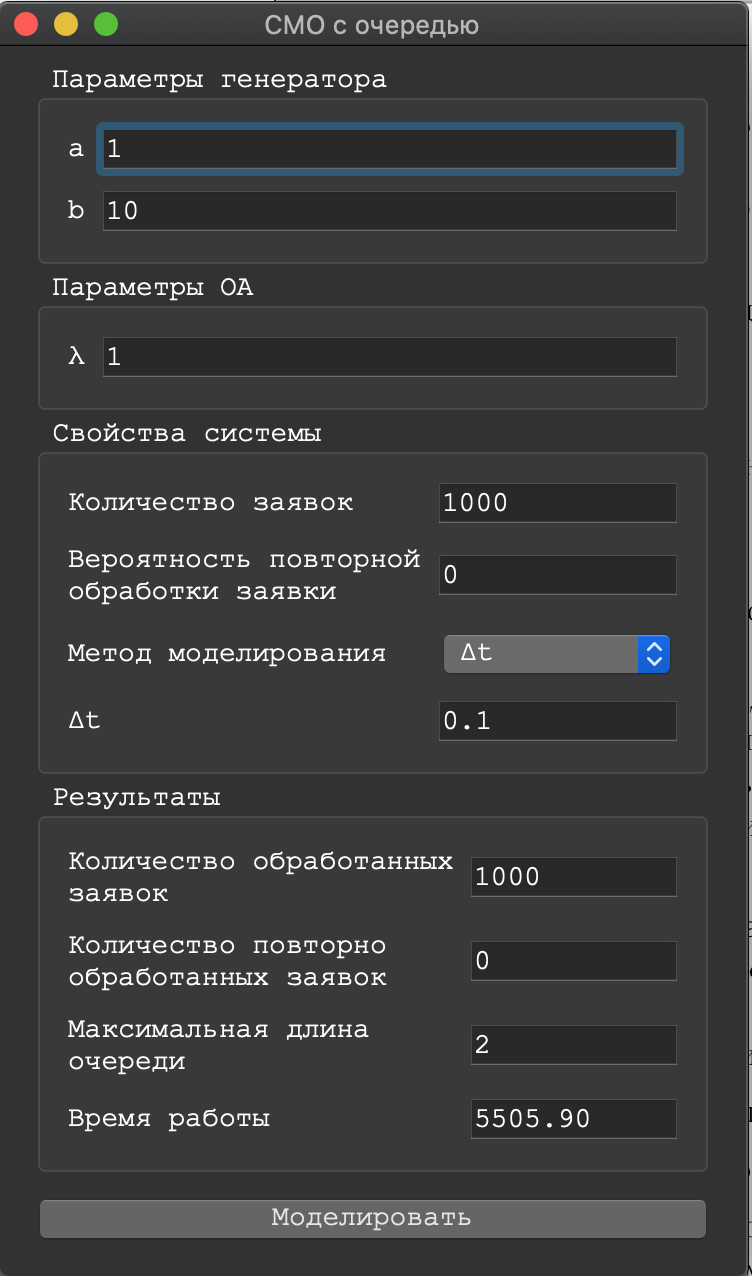
\includegraphics[width=\textwidth]{deltat_1_1.png}
		\end{minipage}
		\begin{minipage}[b]{0.32\textwidth}
			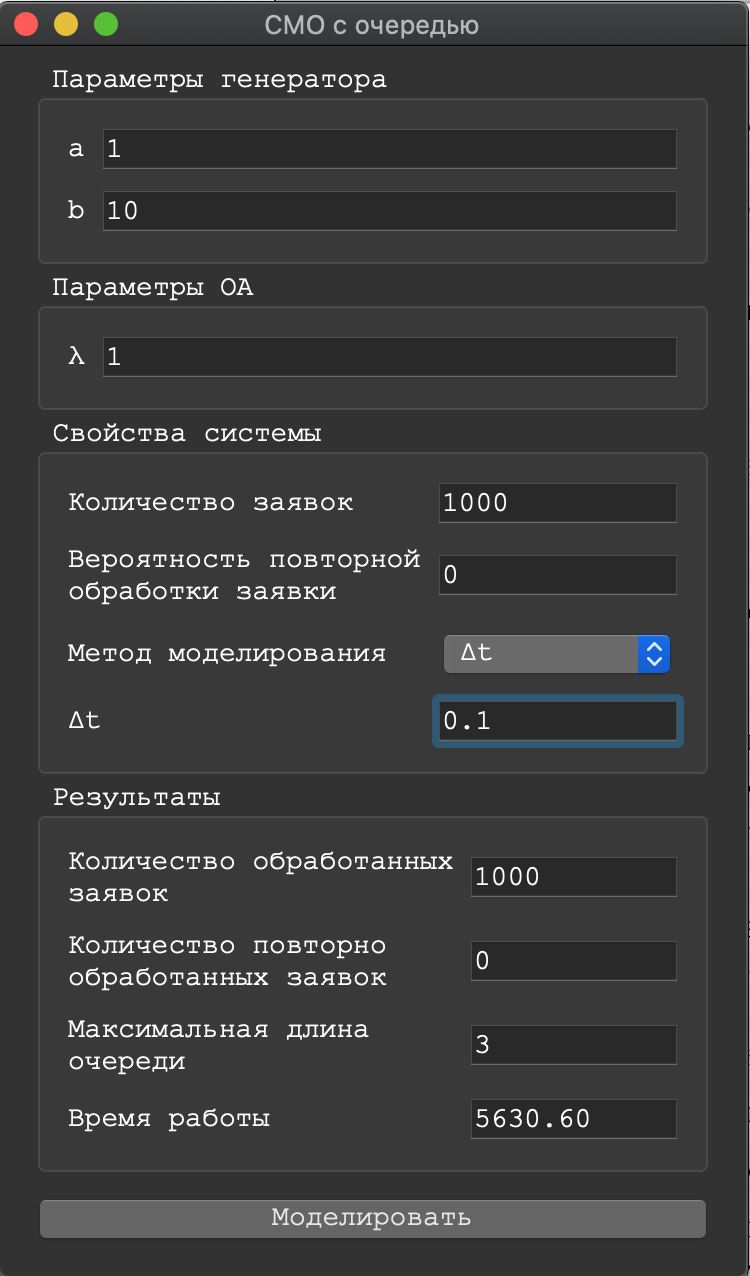
\includegraphics[width=\textwidth]{deltat_1_2.png}
		\end{minipage}
		\begin{minipage}[b]{0.32\textwidth}
			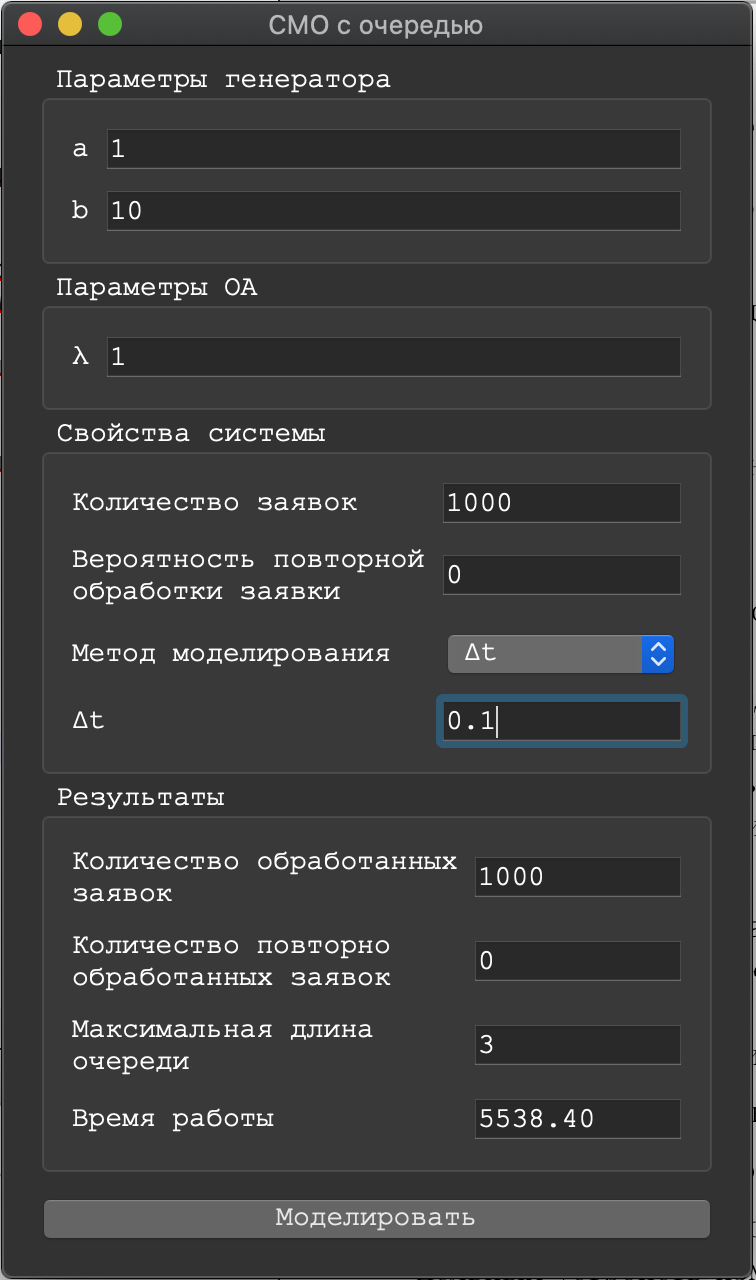
\includegraphics[width=\textwidth]{deltat_1_3.png}
		\end{minipage}
		\center{$\Delta t$ метод. $\Delta t = 0.1$}
		\label{ris:deltat_1}
	\end{figure}

	\begin{figure}[h!]
		\begin{minipage}[b]{0.32\textwidth}
			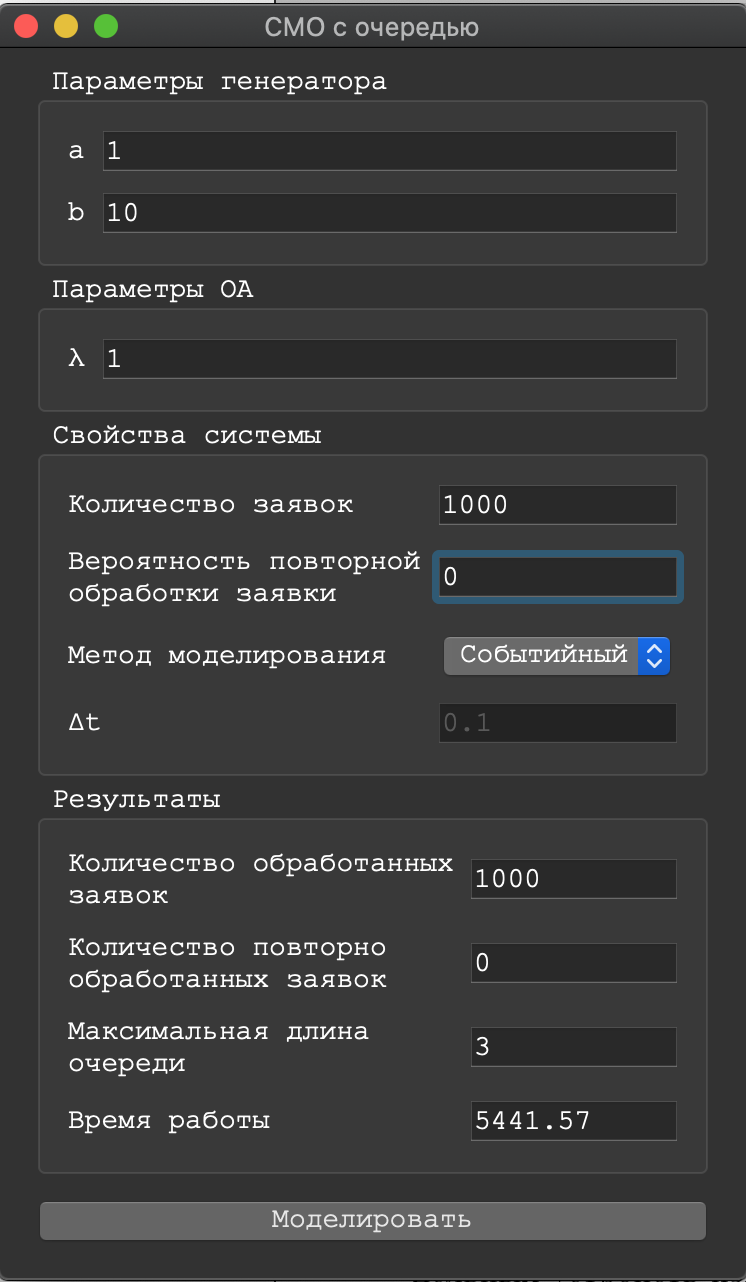
\includegraphics[width=\textwidth]{sob_1_1.png}
		\end{minipage}
		\begin{minipage}[b]{0.32\textwidth}
			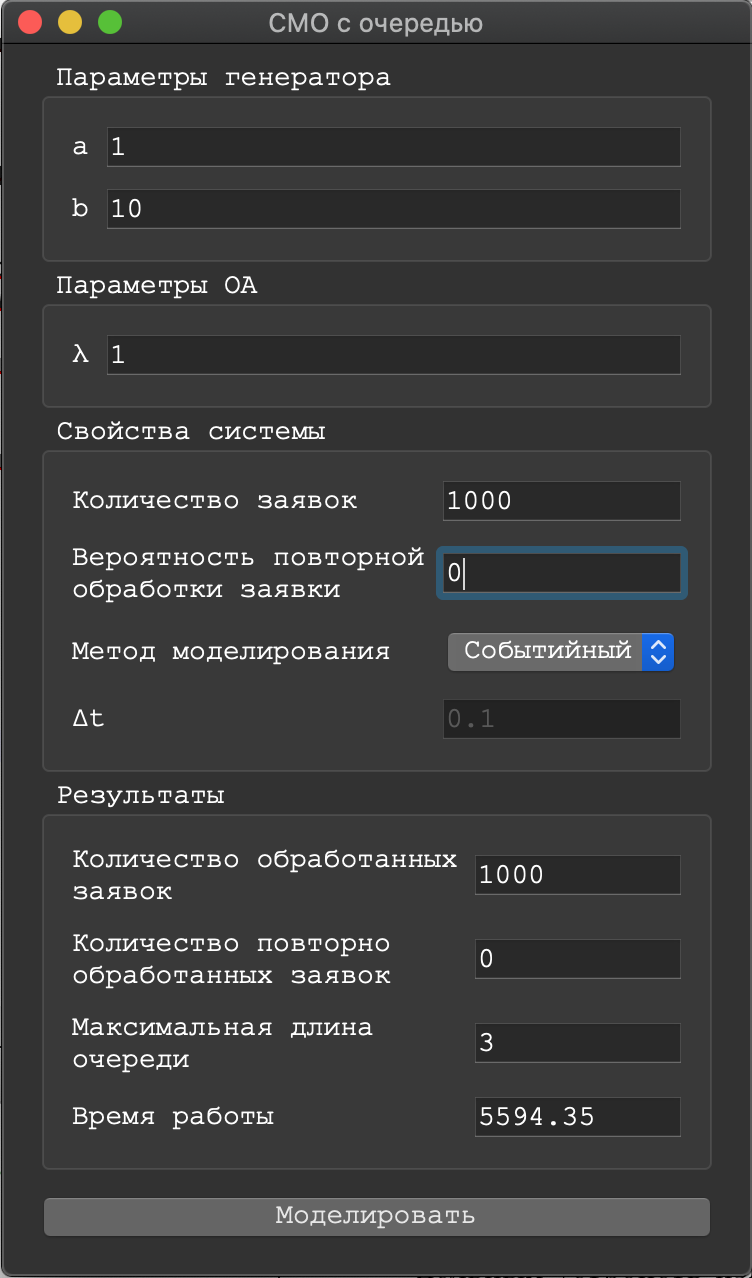
\includegraphics[width=\textwidth]{sob_1_2.png}
		\end{minipage}
		\begin{minipage}[b]{0.32\textwidth}
			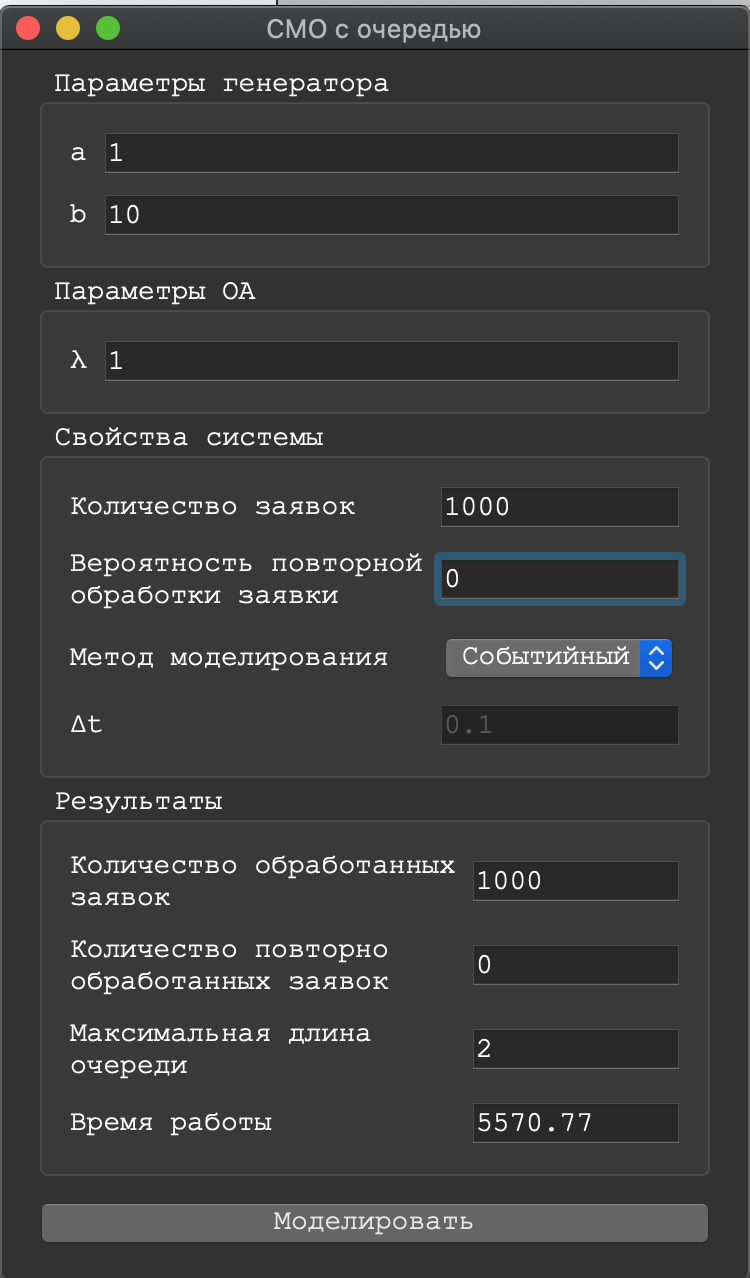
\includegraphics[width=\textwidth]{sob_1_3.png}
		\end{minipage}
		\center{Событийный метод.}
		\label{ris:sob_1}
	\end{figure}

	Видно, что время работы программы и максимальная длина очереди не сильно различаются.
	
	Проведя более 40 повторных опытов при заданных параметрах, было установлено, что максимальноя длина очереди не превышала размера равного 4.
	
	Таким образом, оптимальная длина очереди $L$ при заданных параметрах равна 4.
	
	\newpage
	
	Если же при использовании метода $\Delta t$ задать величину $\Delta t > b$, то программа будет выдавать максимальную длину очереди не больше 1.
	
	\begin{figure}[h!]
		\begin{center}
			{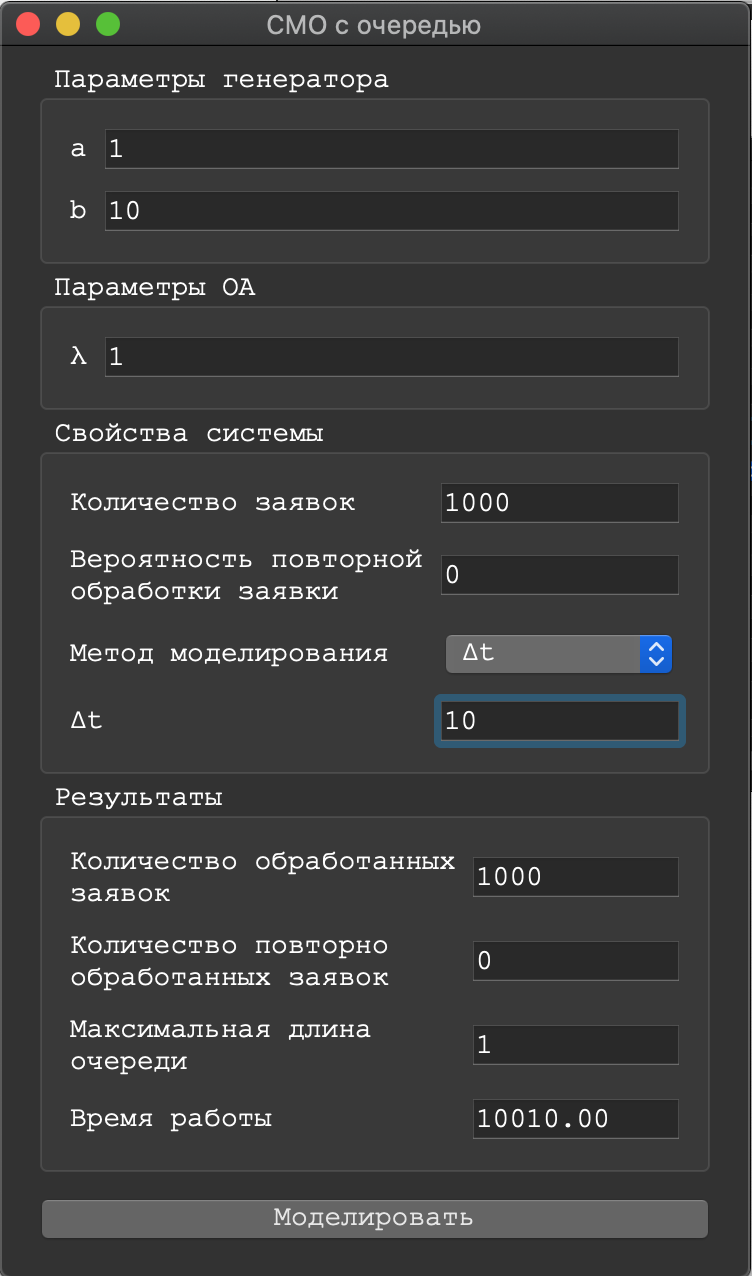
\includegraphics[scale = 0.6]{deltat_2.png}}
			\label{ris:deltat_2}
		\end{center}
		\caption{$\Delta t$ метод. $\Delta t = 0.1$.}
	\end{figure}
	
	Это связано с тем, что и генератор, и Обслуживающий Аппарат, не будут простаивать на каждой итерации, поскольку будут способны выдавать и обрабатывать заявки за время, не превышающее $\Delta t$.
	
	\newpage
	
	Если же задать задать вероятность повторной обработки заявки, равной 0.5, то оптимальная длина очереди $L$ увеличится до 8, поскольку создается дополнительная нагрузка на Обслуживающий Аппарат из-за вновь поступивших в очередь заявок.
	
	\begin{figure}[h!]
		\begin{minipage}[b]{0.32\textwidth}
			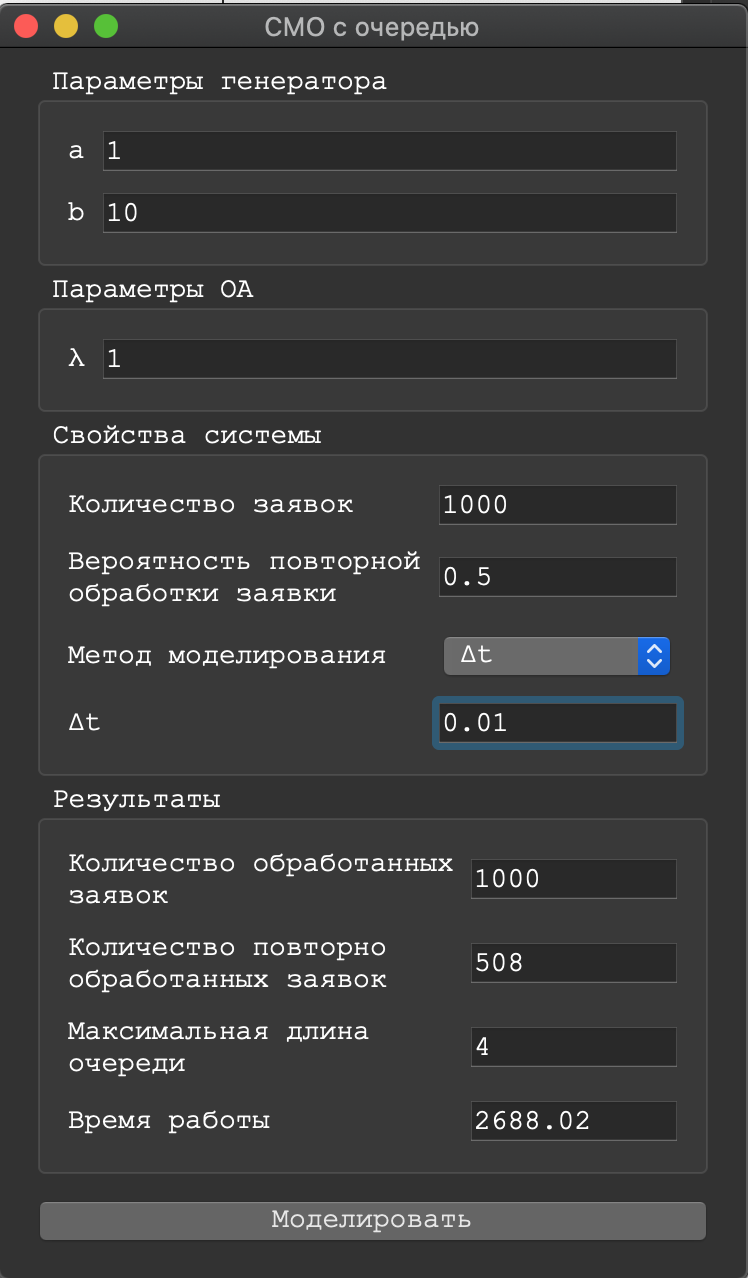
\includegraphics[width=\textwidth]{deltat_3_1.png}
		\end{minipage}
		\begin{minipage}[b]{0.32\textwidth}
			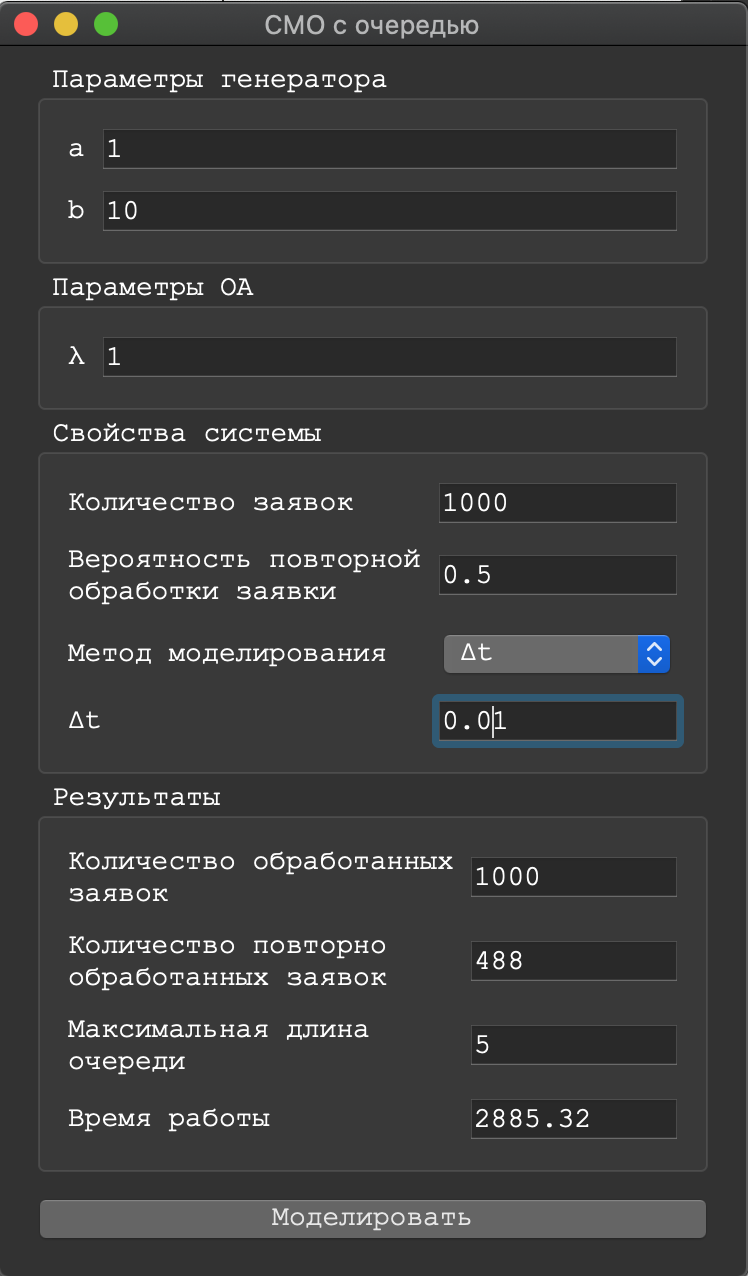
\includegraphics[width=\textwidth]{deltat_3_2.png}
		\end{minipage}
		\begin{minipage}[b]{0.32\textwidth}
			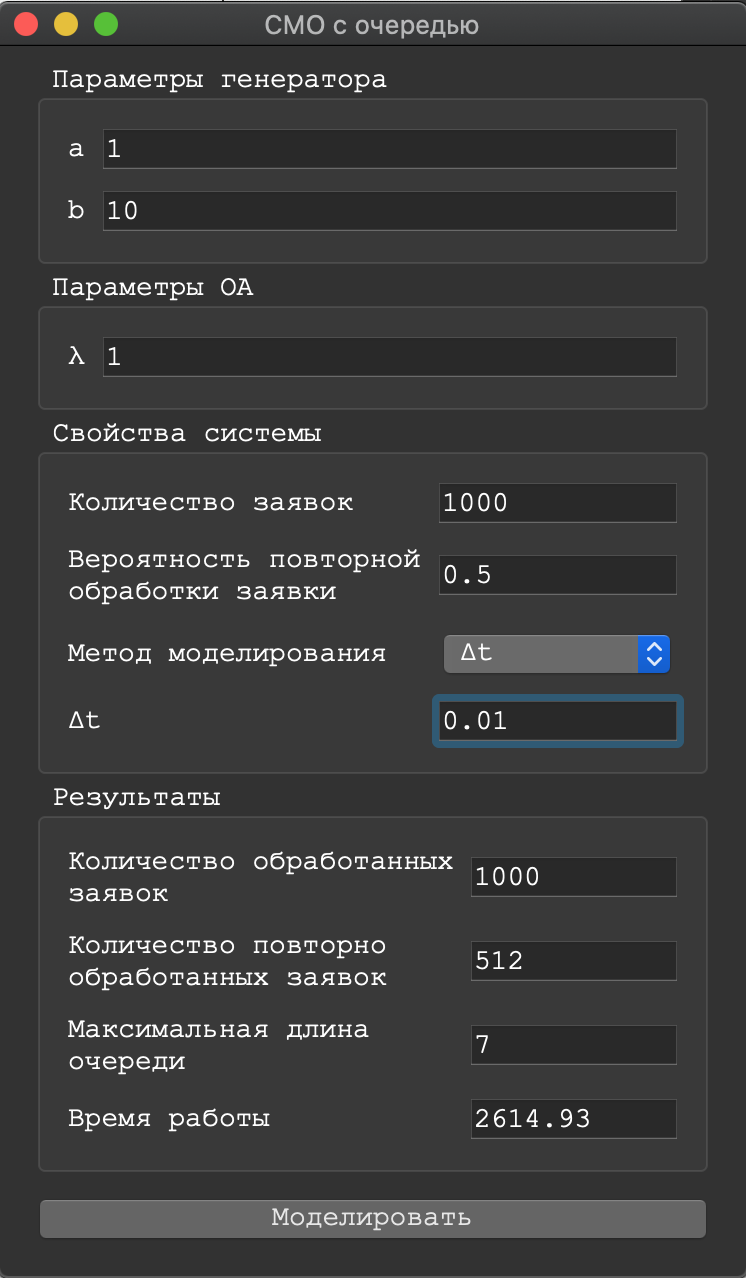
\includegraphics[width=\textwidth]{deltat_3_3.png}
		\end{minipage}
		\center{$\Delta t$ метод. $\Delta t = 0.01$}
		\label{ris:deltat_3}
	\end{figure}
	
	\begin{figure}[h!]
		\begin{minipage}[b]{0.32\textwidth}
			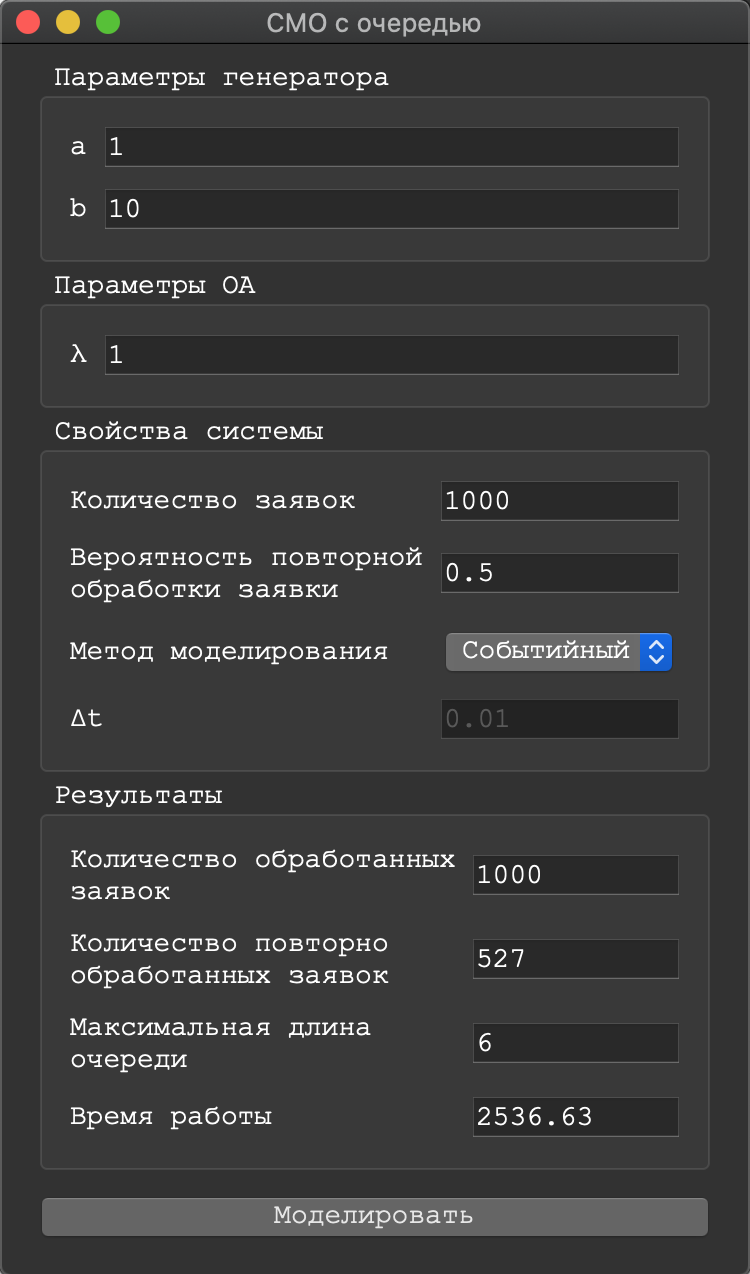
\includegraphics[width=\textwidth]{sob_3_1.png}
		\end{minipage}
		\begin{minipage}[b]{0.32\textwidth}
			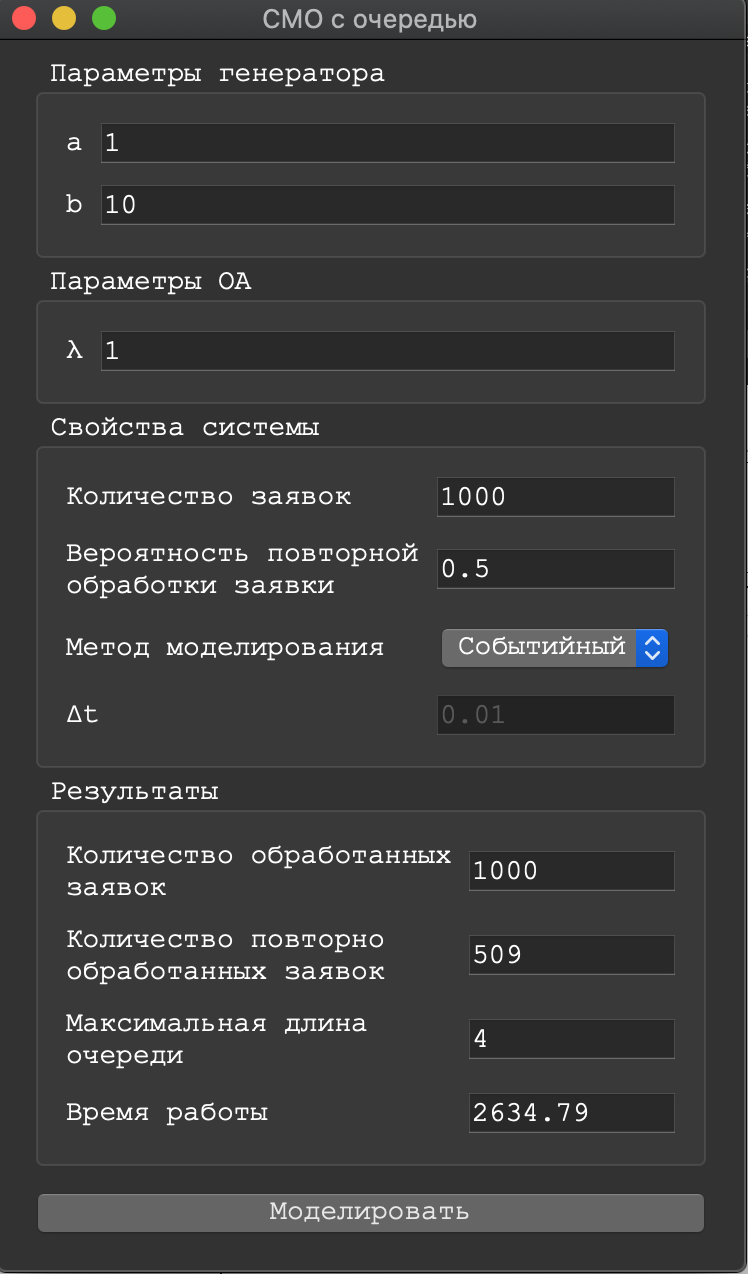
\includegraphics[width=\textwidth]{sob_3_2.png}
		\end{minipage}
		\begin{minipage}[b]{0.32\textwidth}
			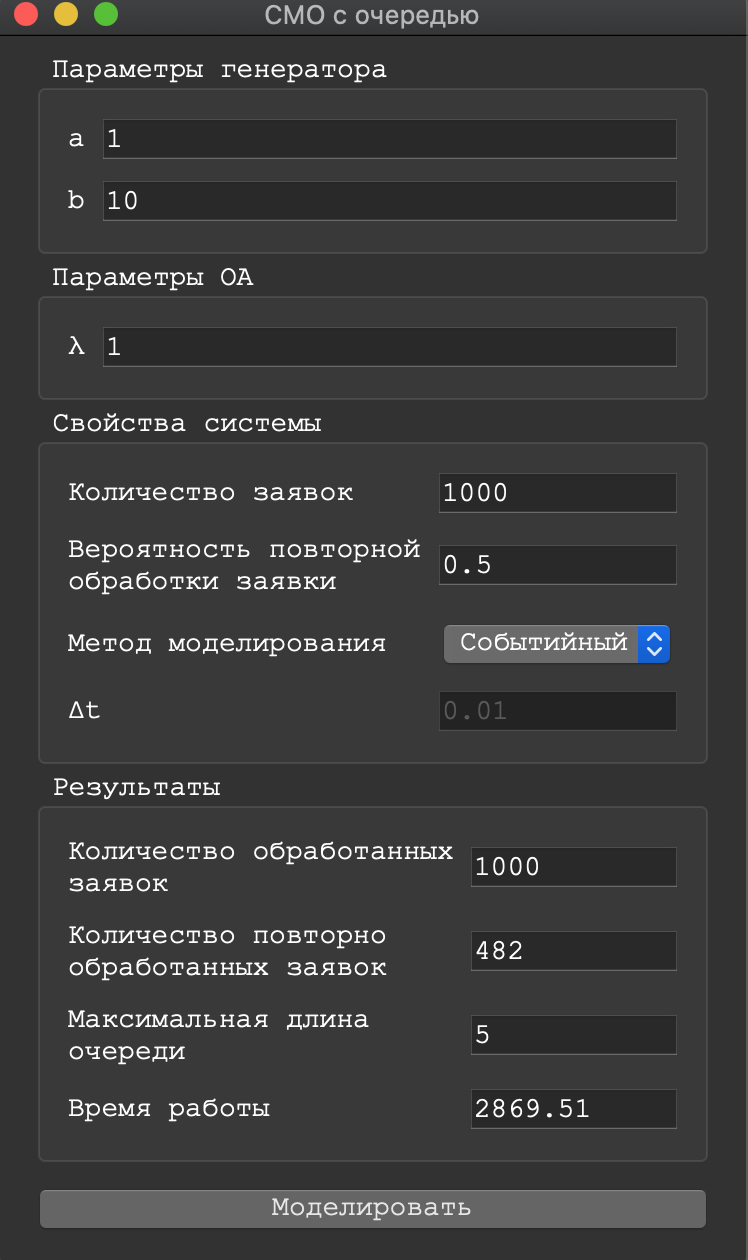
\includegraphics[width=\textwidth]{sob_3_3.png}
		\end{minipage}
		\center{Событийный метод.}
		\label{ris:sob_3}
	\end{figure}

	\newpage
	
	\section*{Вывод}
	
	В результате проделанной работы была дана теоретическая справка по моделированию работы обслуживающего аппарата и проведена формализация задачи.
	
	Была реализована программа, реализующая поставленную задачу.
	
	Были экспериментально подтверждены недостатки принципа $\Delta t$, а именно - значительные затраты машинного времени на реализацию моделирования системы, а также при недостаточно малом $\Delta t$ появляется опасность пропуска отдельных событий в системе, что исключает возможность получения адекватных результатов при моделировании.
	
	Таким образом, для сложных дискретных систем лучше всего стоит применять комбинированный метод при котором на пиковых интервалах он приближается к методу $\Delta t$, а вне - к событийному принципу с большим шагом.
	
\end{document}
	
	